\documentclass{standalone}
\usepackage{pgfplots}
\usepackage{tikz}

\pgfplotsset{
    dirac/.style={
        mark=triangle*,
        mark options={scale=1.5},
        ycomb,
        scatter,
        visualization depends on={y/abs(y)-1 \as \sign},
        scatter/@pre marker code/.code={\scope[rotate=90*\sign,yshift=-2pt]}
    }
}

\pgfplotsset{
    standard/.style={%Axis format configuration
        %axis equal,
        axis x line=middle,
        axis y line=middle,
        minor tick num=1,
        grid=both,
        %enlarge x limits=0.15,
        %enlarge y limits=0.15,
        every axis x label/.style={at={(ticklabel* cs:1.05)},anchor=west},
        every axis y label/.style={at={(ticklabel* cs:1.05)},anchor=south},
        }
}

\begin{document}
    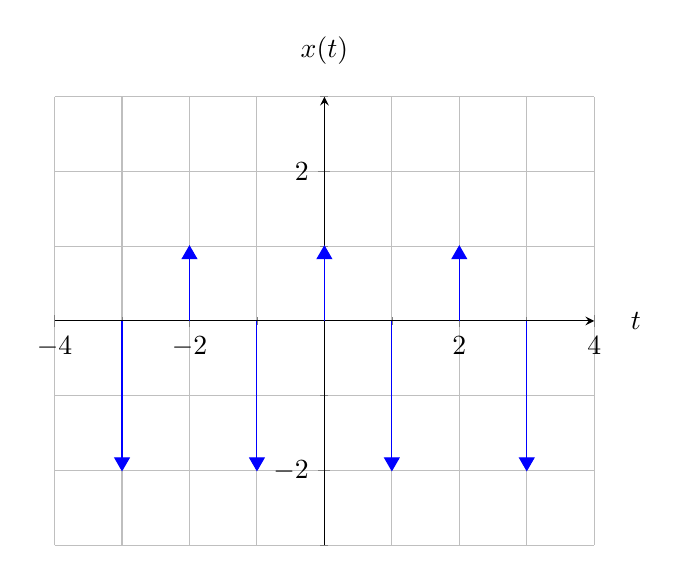
\begin{tikzpicture}
        \makeatletter
        \begin{axis}[standard,xmin=-4,xmax=4,ymin=-3,ymax=3,xlabel={$t$},ylabel={$x(t)$}]
            \addplot +[dirac] coordinates {(-3,-2) (-2,1) (-1,-2) (0,1) (1,-2) (2,1) (3,-2) };
        \end{axis}
    \end{tikzpicture}
\end{document}
